% ================================================
% =                 EXPERIMENTS                  = 
% ================================================ 

This section includes all experiments carried out for evaluating the difference between the two approaches considered in the BEV2Seg\_2 pipeline, experiments to study what is the influence of extrinsic parameters modification as data augmentation technique for semantic segmentation of BEV images and the final evaluation of the proposed annotation pipeline of occupancy, occlusion and driveable areas.

\subsection{BEV2Seg\_2}
Both models, first segmenting-then-IPM and IPM-then-segmenting approaches, has considered the same conditions: no se han congelado las capas del encoder para realizar el fine-tuning en el task de segmentación y el preprocesado de las imágenes se ha realizado con \textit{SegformerImageProcessor} aplicando un cambio de tamaño de la imagen a $512 \times 512$, un re-escalado con un factor de $1/255$ y un normalizado con los valores de media y desviación típica de ImageNet. De esta forma, aseguramos que el preprocesado realizado es el mismo que el esperado por los encoders. 

Además, a la hora de proporcionar las máscaras semánticas de entrenamiento, el parámetro "reduce\_labels" se ha mantenido en \textit{False}, ya que no contamos con la clase "background". Aquellas zonas que no se quieren inferir, como son el fondo y las áreas no etiquetadas, tienen el label "ignore" así que no se calcula gradiente para ellas.

All the experiments were carried out with the hardware shown in Table \ref{tab:hardware}


The notation of models following the first segmenting then IPM for obtaining the BEV semantic masks has been named as "raw2seg\_bev" while the IPM and then segmenting approach has been named as "raw2bev\_seg". Three out of six Segformer's encoder sizes has been selected: MiT-b0, MiT-b2 and MiT-b4.

\begin{table}[h]
    \centering
    \begin{tabular}{c l c}
        \toprule
        \textbf{Component} & \textbf{Specifications} & \textbf{Num workers} \\
        \midrule
        CPU         & - & 8 \\
        GPU         & - & 2 \\      
        Memmory     & - & - \\
        OS          & - & - \\
        \bottomrule
    \end{tabular}
    \caption{ Hardware used for experiments }
    \label{tab:hardware}
\end{table}

The two approaches were first trained in model size MiT-b0 for $20,7K$ steps without any regularization technique being applyed. The idea of this first experiment was to see if the models suffers from overfitting, so the smallest model size was used as they are fastest to train, it more unlike to has an extreme overfitting as its capacity for "remembering" and adjusting to training data is less than bigger models (although they can suffer from underfitting) and it is a good environment to test hyperparamenters configurations.


With this configuration the results shown in figure \ref{fig:overfitting_mit-b0} were a clear overfitting of the two approaches can be seen as while the training loss continues decreasing, the evaluation loss starts increasing without showing a clear convergence. Seeing this results with the lightweigtest segformer's model enhances the idea of applying regularization techniques during training. 

Thats why, the data augmentation techniques described in \ref{data_augmentations} where employed to train the models with varying data and other regularization techniques such as weight decay, or L2 regularization, were employed. \hl{Explain weight decay briefly}. With the use of this regularization techniques, the overfitting was reduced


Importante destacar que durante las evaluaciones, los conjuntos de evaluacion son distintos: un pipeline evala sobre BEV y otro sobre normal, de ahí la diferencia significativa entre ambos. También, destacar que es posible que haya underfitting ya que el mIoU se mantiene bastante bajo.


\hl{I didn't find what is the segformer's loss function.}

\hl{Comment that with model size MiT-b4 gradient accumulation techniques were used to fit the GPU memory specs.}

\hl{Comment the max epochs set to 200 and the checkpoint strategy used: it is controvesial wheter to use the loss or mIoU. Whe have decided to use the loss.}



\begin{figure}[h!]
    \centering
    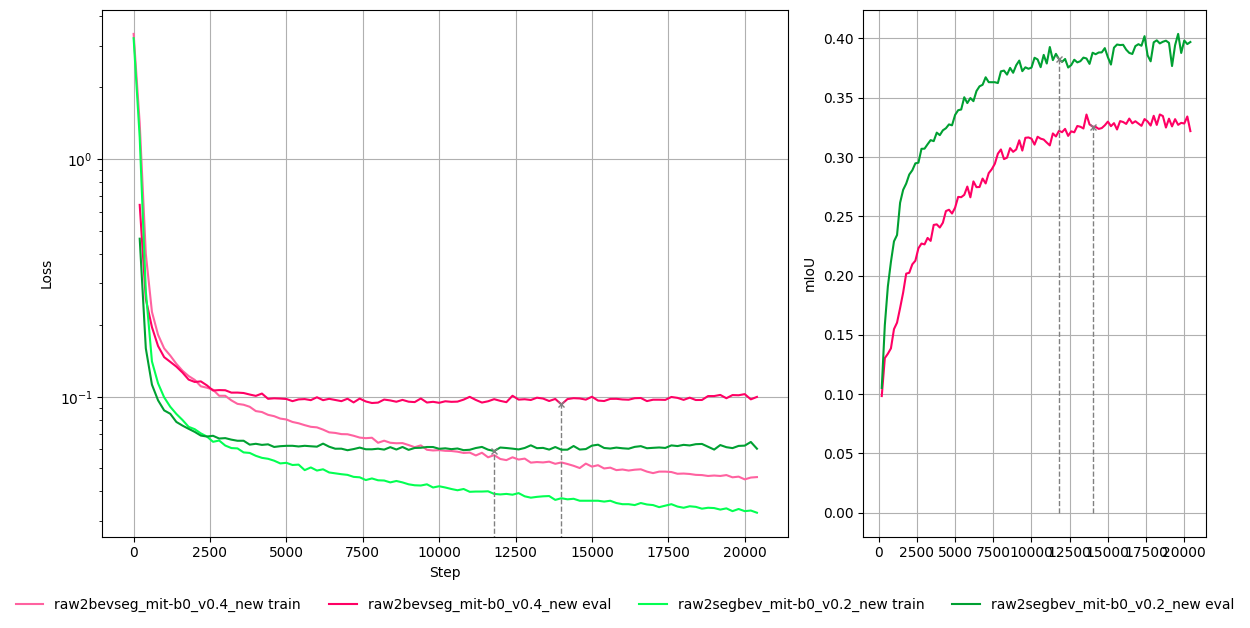
\includegraphics[width=\linewidth]{./images/experiments/overfitting_bev_nu.png}
    \caption{Training and evaluation loss of raw2seg\_bev and raw2bev\_seg MiT-b0 models without any regularization technique}
    \label{fig:overfitting_mit-b0}
\end{figure}



\subsubsection{BEV images data augmentation techniques comparison}
\hl{Comparison between normal geometric data augmentation techniques and camera's extrinsic parameters modifications.}


\subsubsection{Pipeline comparison}
\hl{raw2seg\_bev results compared with raw2bev\_seg results.}

\subsection{3D detections evaluations}
\hl{Explain the selected NuScenes selected vehicle scene, and expose the metrics used (mIoU and v2v distance).}

\subsection{BEV masks evaluation}
\hl{Groundtruth BEV masks could be generated from annotations and compute mIoU between the annotated BEV masks and ground truth ones.}

